\documentclass[pdf]{beamer}
\mode<presentation>{}
\usepackage{minted}
\usepackage{tikz}
\usepackage{pgffor} %% gives looping with \foreach
\usepackage[absolute,overlay]{textpos}
\usepackage{lmodern} %% scalable latin characters
\usetikzlibrary{arrows,shapes,backgrounds}
\usepackage{multirow}
\usepackage{listings} %% another package for code related stuff

%% stuff for minted
\definecolor{mintedBg}{rgb}{0.95, 0.95, 0.95}
\definecolor{blockBg}{rgb}{0.6, 0.6, 0.95}
\definecolor{rnaColor}{rgb}{0, 0.6, 0}
\definecolor{cdsColor}{rgb}{0, 0.4, 0.4}
\definecolor{rnaPol}{rgb}{0.8,0,0.8}
\definecolor{ribosomeCol}{rgb}{0.5,0.5,0.1}
\definecolor{protColor}{rgb}{0.6,0,0.6}
%% colours for nucleotides:
\definecolor{dACol}{rgb}{0.5, 0.5, 0}
\definecolor{dCCol}{rgb}{0.8, 0, 0}
\definecolor{dGCol}{rgb}{0, 0.8, 0}
\definecolor{dTCol}{rgb}{0, 0, 0.8}

\definecolor{navy}{rgb}{0, 0, 0.6}
\definecolor{pur}{rgb}{0, 0, 0.6}
\definecolor{pyr}{rgb}{0.6, 0, 0.2}
%% define styles for different codes
\newminted{cpp}{linenos, bgcolor=blockBg, fontsize=\footnotesize}
%% then use \begin{cppcode}
\newminted{c}{linenos, bgcolor=mintedBg, fontsize=\footnotesize}
\newminted{perl}{linenos, bgcolor=mintedBg, fontsize=\footnotesize}
\newminted{sql}{linenos, bgcolor=mintedBg, fontsize=\footnotesize}

%% a command to define a subheading
\newcommand\subHeading[1]{
  \par\bigskip {\Large\bfseries#1}\par\smallskip
}

%% I detest indentation in footnotes etc, so try this:
\makeatletter
\renewcommand\@makefntext[1]{\noindent\makebox[0em][r]{\@makefnmark}\tiny#1}
\makeatother
%% the makeatletter and makeatother are required to allow me to
%% to change the macro beginning with an @. (though when I call it
%% I don't use the @ ... 

\setlength\parskip{0.5em}
\setlength\parindent{0ex}

%% to have footnotes without references. This from tex.stackexchange.com
\newcommand\blfootnote[1]{%
  \begingroup  %% this makes it a local redefinition
  \renewcommand\thefootnote{}\footnote{#1}%
  \addtocounter{footnote}{-1}  % this adjusts the footnote counter
  \endgroup
}

%% a command for drawing a ribosome structure
%% as two circles
\newcommand{\riboS}[3][0.8]{
  \draw[fill=ribosomeCol] (#2,#3-#1) circle [radius=#1];
  \draw[fill=ribosomeCol] (#2,#3+#1/1.5) circle [radius=#1/1.5];
}

%% a command to draw a protein at a given location:
\newcommand{\protein}[2]{
  \draw[protColor, line width=1] (#1,#2) to [out=180, in=45] (#1-1.5,#2-1)
  to [out=225, in=270] (#1-0.5,#2-2) to [out=270-180, in=330] (#1-1,#2-1.25)
  to [out=330-180, in=90] (#1-2,#2-1)
  to [out=250, in=180] (#1, #2-2);
  \draw[protColor, line width=4, dotted] (#1,#2) to [out=180, in=45] (#1-1.5,#2-1)
  to [out=225, in=270] (#1-0.5, #2-2) to [out=270-180, in=330] (#1-1, #2-1.25)
  to [out=330-180, in=90] (#1-2, #2-1)
  to [out=250, in=180] (#1, #2-2);
}


\title{Databases}
\subtitle{Structuring data}
\author{Martin Jakt}

\begin{document}

\begin{frame}
  \titlepage
\end{frame}

\begin{frame}{What is a database?}
  In its simplest form:\\
  \textcolor{navy}{A collection of data in some defined format}
  \pause
  \begin{itemize}
  \item Flat files
  \item Relational
  \item Object orientated
  \end{itemize}

  \pause
  We will be primarily concerned with relational, but first..

  \visible<2->{
    \blfootnote{There are some others as well, but these are the main types}
  }

\end{frame}

\begin{frame}{Flat files}
No specific requirements but the data in the files should follow 
some predefined specification describing the encoding and organisation
of the data.

Some examples:
\begin{description}
\item[Sequences] A collection of fasta files, or a single multisequence fasta file
\item[Expression] A collection of Soft format files
\item[Images] A collection of jpegs
\end{description}

Easy to create, difficult to query (eg. need to read all files to get all sequence names or lengths).

Good for genome sequences (but not the annotation).
\end{frame}

\begin{frame}{Object orientated}
  \begin{itemize}
  \item Data is structured into classes
  \item Objects are instances of classes
  \item Objects are collections of other objects
  \end{itemize}
\end{frame}

\begin{frame}{Object orientated}
  For example: A gene can be represented by a class that contains:
  \begin{itemize}
  \item Promoter
  \item Splice site acceptors
  \item Splice site donors
  \item polyA signal
  \item Transcripts
  \end{itemize}
  
  Where Promoter, Splice site acceptors themselves are objects of their own right.
  
  Object orientated databases are more flexible in the types of data
  that they can represent (esp. tree like) but trade off flexibility
  in querying for speed.

  Suitable for big and or complicated data-sets?
\end{frame}

\begin{frame}{Relational}
  \begin{itemize}
  \item provides a framework for storing data in a structured manner
  \item provides mechanisms for ensuring data integrity
  \item based on well understood\footnote{by discrete mathematicians} discrete mathematics
  \end{itemize}
  \pause
  But what does that mean?
\end{frame}

\begin{frame}{Typical experimental data}
%  pgfversion is \pgfversion
  \begin{figure}[ht]
    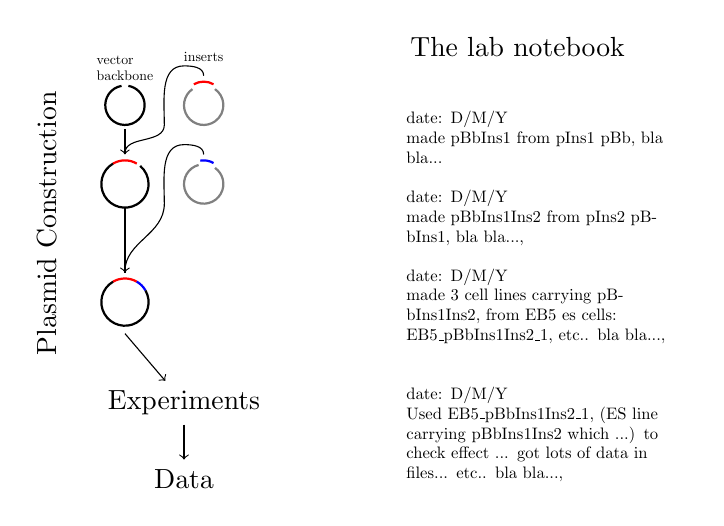
\begin{tikzpicture}[scale=0.5]
%      \draw [help lines, opacity=1] (0,0) grid (22,12);
%      \foreach \x in {1,2,...,20} \node [font=\small] at (\x,0) {\x};
%      \foreach \y in {1,2,...,11} \node [font=\small] at (20,\y) {\y};
      
      \node [above, rotate=90] at (-1.5,7) {Plasmid Construction};

      \visible<1->{
      \draw [-, black, thick] (0,10) ++(90+10:0.5) arc((90+10):(360+90-10):0.5);
      \draw [-, gray, thick] (2,10) ++(90+35:0.5) arc((90+35):(360+90-35)):0.5); 
      \draw [-, red, thick] (2,10.1) ++(90+30:0.5) arc((90+30):(90-30)):0.5); 
      
      \draw [->] (2,10.75) to [out=90,in=0] (1.5,11)
            to [out=180,in=90] (1,9.5)
            to [out=270,in=90] (0,8.75);
      \draw [-] (0,9.4) -- (0,8.75); 
      

%      \draw [-, black, thick] (1,8) ++(90+30:0.6) arc((90+30):(360+90-30)):0.6); 
%      \draw [-, red, thick] (1,8) ++(90+30:0.6) arc((90+30):(90-30)):0.6); 
      \draw [-, black, thick] (0,8) ++(90+30:0.6) arc((90+30):(360+90-40)):0.6); 
      \draw [-, red, thick] (0,8) ++(90+30:0.6) arc((90+30):(90-30)):0.6); 
      }
      \visible<2->{
      \draw [-, gray, thick] (2,8) ++(90+15:0.5) arc((90+15):(360+90-35)):0.5); 
      \draw [-, blue, thick] (2,8.1) ++(90+10:0.5) arc((90+10):(90-30)):0.5); 

      \draw [->] (2,8.75) to [out=90,in=0] (1.5,9)
            to [out=180,in=90] (1,7.5)
            to [out=270,in=90] (0,5.75);
      \draw [-] (0,7.4) -- (0,5.75); 
            
      \draw [-, black, thick] (0,5) ++(90+30:0.6) arc((90+30):(360+90-60)):0.6); 
      \draw [-, red, thick] (0,5) ++(90+30:0.6) arc((90+30):(90-30):0.6); 
      \draw [-, blue, thick] (0,5) ++(90-30:0.6) arc((90-30):(90-60):0.6); 
      }

      \node [above, align=left, scale=0.5] at (0,10.5) {vector\\backbone};
      \node [above, align=left, scale=0.5] at (2,11) {inserts};

      \visible<3->{
      \node [below] (e1) at (1.5,3) {Experiments};
      \node [below] (d1) at (1.5,1) {Data};
      \draw [->] (e1) -- (d1);
      \draw [->] (0,4.2) -- (e1);
    }
      
      %% how we enter this;;;
    \visible<4->{
      \node [above right] at (7,11) {The lab notebook};
      \node [below right, align=left, text width=6 cm, scale=0.6] at (7,10)
      {date: D/M/Y\\made pBbIns1 from pIns1 pBb, bla bla...};

      \node [below right, align=left, text width=6 cm, scale=0.6] at (7,8)
      {date: D/M/Y\\made pBbIns1Ins2 from pIns2 pBbIns1, bla bla..., };

      \node [below right, align=left, text width=6 cm, scale=0.6] at (7,6)
      {date: D/M/Y\\made 3 cell lines carrying pBbIns1Ins2, 
       from EB5 es cells: EB5\_pBbIns1Ins2\_1, etc.. bla bla..., };

      \node [below right, align=left, text width=6 cm, scale=0.6] at (7,3)
      {date: D/M/Y\\Used EB5\_pBbIns1Ins2\_1, (ES line carrying pBbIns1Ins2
        which ...) to check effect ... got lots of data in files... etc.. bla bla...,};
}
      

    \end{tikzpicture}
  \end{figure}
\end{frame}

\begin{frame}{so what?}
  All the data describing the experiments is in the note book. But...
  \begin{itemize}
  \item Description of reagents (plasmids) is dispersed.
  \item Individual reagent descriptions are dispersed (step 1: a year ago
    , step 2: a month ago, step 3: last week)
  \item Long reagent names (difficult to label tubes).
  \item Descriptions of reagents are repeated to make experiment descriptions
    readable.
    \begin{itemize}
      \item $\Rightarrow$ conflicting descriptions possible.
    \end{itemize}
  \end{itemize}
\end{frame}

\begin{frame}{a big mess}
  In the lab, the biggest problem is probably how to label tubes.
  \pause

  So what to do:
  \begin{enumerate}
  \item Use a single unique number that always increases to identify plasmids.
  \item Label tubes with this number.
  \item Keep a record of plasmids in a separate notebook.
  \item Refer to plasmids by number in experimental description.
  \item Do the same for cell lines, animals, etc...
  \end{enumerate}

  This is the essence of a relational database.\\
  No need for a computer.
\end{frame}

\begin{frame}{the lab relational db}
  So what's good about that then?
  \begin{itemize}
  \item Easy to find information about any reagent, as
    they are now stored in a sorted list (your plasmid/ cell line/ etc... book).
  \item Easy to modify descriptions if necessary (as the description
    is in one place only).
  \item No conflicting descriptions.
  \item Easy to label / identify tubes in the freezer.
  \end{itemize}
  \blfootnote{There are more details to making a convenient lab record, but
    that would be too much detail for this course}
\end{frame}

\begin{frame}{books to computers}
  books $\rightarrow$ tables\\
  1 entry $\rightarrow$ 1 row\\
  1 column $\rightarrow$ 1 property of entries 

  \pause
  How many tables do we need to describe the data?\\
  Depends on the relationships between the objects we describe.

  \begin{tabular}{lcl}
%  \begin{itemize}
    \textcolor{navy}{one to one} & $\rightarrow$  & one table\\
    \textcolor{navy}{one to many} & $\rightarrow$ & two tables\\
    \textcolor{navy}{many to many} & $\rightarrow$ & three tables \\
    % \end{itemize}
  \end{tabular}

  \pause
  The aim is to represent the data in an extensible way that minimises
  the number of tables and ensures that data points are only recorded
  at one location.
  \blfootnote{many can also include 0, i.e. it's an unspecified number}
\end{frame}

\begin{frame}{A simplified experimental database}
  We have:

  \begin{tabular}{p{0.2\linewidth}|p{0.5\linewidth}}
  thing & data about the thing \\
  \hline
  plasmids & identifier (numeric), what (text), how (text) and when (date) \\
  cell lines & identifier (numeric), what (text) how (text) and when (date), 
  plasmids included (numeric) \\
  experiments & identifier (numeric), what (text), how (text), when (date),
  cell lines\\
  \end{tabular}

\end{frame}

\begin{frame}{The implementation}
  \begin{figure}[ht]
    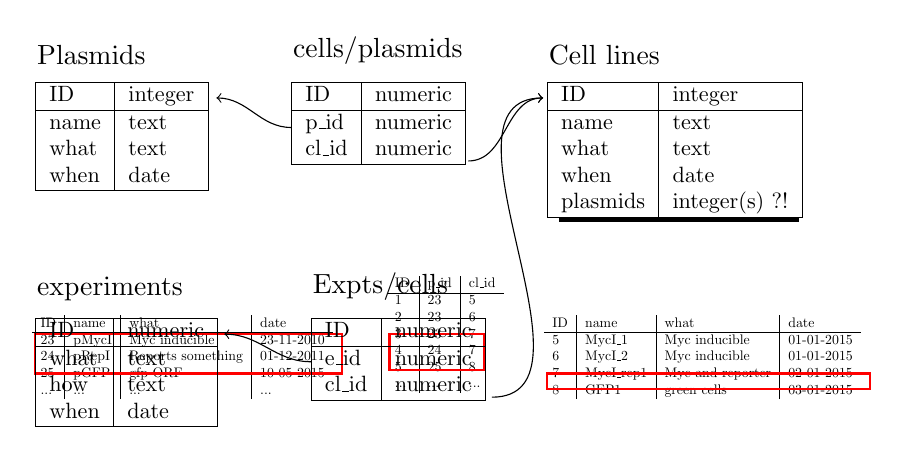
\begin{tikzpicture}[scale=0.5]
%      \draw [help lines, opacity=1] (0,0) grid (22,12);
%      \foreach \x in {1,2,...,20} \node [font=\small] at (\x,0) {\x};
%      \foreach \y in {1,2,...,11} \node [font=\small] at (20,\y) {\y};
      
      \visible<1->{
        \node [below right, align=left, scale=0.8]
        (p1) at (0,11) {
          \begin{tabular}{|l|l|}
            \hline
            ID & integer \\
            \hline
            name & text \\
            what & text \\
            when & date \\
            \hline
          \end{tabular} };
        \node [above right] at (0,11) {Plasmids};
      }
      \visible<2->{
        \node [below right, align=left, scale=0.8]
        (cl1) at (13,11) {
          \begin{tabular}{|l|l|}
            \hline
            ID & integer \\
            \hline
            name & text \\
            what & text \\
            when & date \\
            plasmids & integer(s) ?! \\
            \hline
          \end{tabular} };
        \node [above right] at (13,11) {Cell lines};
      }
      \visible<3->{
        \draw [-, ultra thick] (13.5,7.3) -- (19.6,7.3);
      }

      \visible<4->{
        \node [below right, align=left, scale=0.8]
        (pcl1) at (6.5,11) {
          \begin{tabular}{|l|l|}
            \hline
            ID & numeric \\
            \hline
            p\_id & numeric \\
            cl\_id & numeric \\
            \hline
          \end{tabular} };
        \node [above right ] at (6.5,11) {cells/plasmids};
      }
      \visible<5->{
        \draw [->] (6.7,9.65) to [out=180,in=0]
        (4.8,10.4);
        \draw [->] (11.2,8.8) to [out=0, in=180]
        (13.1,10.4);
      }

      \visible<6-8>{
        \node [below right, align=left, scale=0.5]
        at (0,5) {
          \begin{tabular}{l|l|l|l}
            ID & name & what & date \\
            \hline
            23 & pMycI & Myc inducible & 23-11-2010 \\
            24 & pRepI & Reports something & 01-12-2011 \\
            25 & pGFP & gfp ORF & 10-05-2015 \\
            ... & ... & ... & ...\\
          \end{tabular} };
        
        \node [below right, align=left, scale=0.5]
        at (13,5) {
          \begin{tabular}{l|l|l|l}
            ID & name & what & date \\
            \hline
            5 & MycI\_1 & Myc inducible & 01-01-2015 \\
            6 & MycI\_2 & Myc inducible & 01-01-2015 \\
            7 & MycI\_rep1 & Myc and reporter & 02-01-2015 \\
            8 & GFP1 & green cells & 03-01-2015 \\
          \end{tabular} };
      }
      \visible<7-8>{
        \node [below right, align=left, scale=0.5]
        at (9, 6) {
          \begin{tabular}{l|l|l}
            ID & p\_id & cl\_id \\
            \hline
            1 & 23 & 5 \\
            2 & 23 & 6 \\
            3 & 23 & 7 \\
            4 & 24 & 7 \\
            5 & 25 & 8 \\
            ... & ... & ...\\
          \end{tabular} };
      }
      \visible<8>{
        \draw [red, thick] (9.2,3.5) rectangle (11.6,4.4);
        \draw [red, thick] (0.2,3.4) rectangle (8,4.4);
        \draw [red, thick] (13.2, 3) rectangle (21.4,3.4);
      }
      \visible<9->{
        \node [below right, align=left, scale=0.8]
        (e1) at (0,5) {
          \begin{tabular}{|l|l|}
            \hline
            ID & numeric \\
            \hline
            what & text \\
            how & text \\
            when & date \\
            \hline
          \end{tabular} };
        \node [above right] at (0,5) {experiments};
        \node [below right, align=left, scale=0.8]
        (ecl1) at (7,5) {
          \begin{tabular}{|l|l|}
            \hline
            ID & numeric \\
            \hline
            e\_id & numeric \\
            cl\_id & numeric \\
            \hline
          \end{tabular} };
        \node [above right] at (7,5) {Expts/cells};
        \draw [->] (7.2,3.7) to [out=180,in=0] (5,4.4);
        \draw [->] (11.8,2.8) to [out=0, in=180] (13.1,10.4);
      }
    \end{tikzpicture}
  \end{figure}
\end{frame}

\begin{frame}{virtues}
  grossly oversimplified schema, but:
  \begin{itemize}
  \item We can easily make queries across the data to find things like:
    \begin{itemize}
    \item All cells containing a particular plasmid
    \item All experiments using a cell line containing a plasmid
    \item All experiments / plasmids / experiments made or carried out
      within a given period
    \end{itemize}
  \item Ensure that descriptions of plasmids associated with cell lines
    actually exist (no dangling references).
  \end{itemize}
\end{frame}

\begin{frame}{more data}

  {\small
  \begin{itemize}
  \item personal identifiers. It is useful to know who made a
    particular reagent or performed an experiment:
    \begin{itemize}
    \item the holder of additional knowledge
    \item to spot trends in data
    \end{itemize}
    $\Rightarrow$ new \texttt{users} table and additional column in relevant tables
  \item plasmid parents? Single column (single main parent) or a plasmid\_parent table
    (multiple parents)
  \item plasmids contain DNA sequences. Can be linked to external genome databases (complex).
  \item Experiment descriptions probably very repetitive. If sufficiently, can be formalised
    to some stupid level of detail.
  \item Sample metadata (experimental details / half way measures etc...) should be included
    as this facilitates automated analyses.
  \end{itemize}
  }
  but there is no end to this, and the database can get infinitely complex.
\end{frame}

\begin{frame}{inconsistencies}
  A good structure will ensure:
  \begin{itemize}
  \item data consistency (no contradictory data)
  \item data integrity (no missing data)
  \item extensibility / flexibility
  \end{itemize}

  Database cannot gurantee absence of errors in data. 

  But in complex systems small errors are like little lies;\\
  difficult to introduce without also introducing inconsistencies 
  into the narrative.
\end{frame}

\begin{frame}{a confession}
  \pause
  \begin{itemize}
  \item Experiments are very hard to describe formally (too variable!)
    \pause
  \item Creating an interface that doesn't make data entry / modification / 
    lookup a right pain is maybe even more difficult
    \pause
  \item In most cases I would recommend using a collection of notebooks
    rather than spending time with a computer.
  \end{itemize}

  But... there are commercial products that aim to solve this kind of problem, maybe they're OK.
  \pause

  \emph{\bfseries big projects} should formalise their experimental procedures / reagents / data
  in databases.
  
\end{frame}

\begin{frame}{Ensembl core database schema}
  \begin{figure}[ht]
    \includegraphics[width=\textwidth]{images/fundamental_tables_core_crop1}
  \end{figure}
\end{frame}

\begin{frame}{Ensembl more core}
  \begin{figure}[ht]
    \includegraphics[width=\textwidth]{images/fundamental_tables_core_crop2}
  \end{figure}
\end{frame}

\begin{frame}{genes to proteins}
  \begin{figure}[ht]
    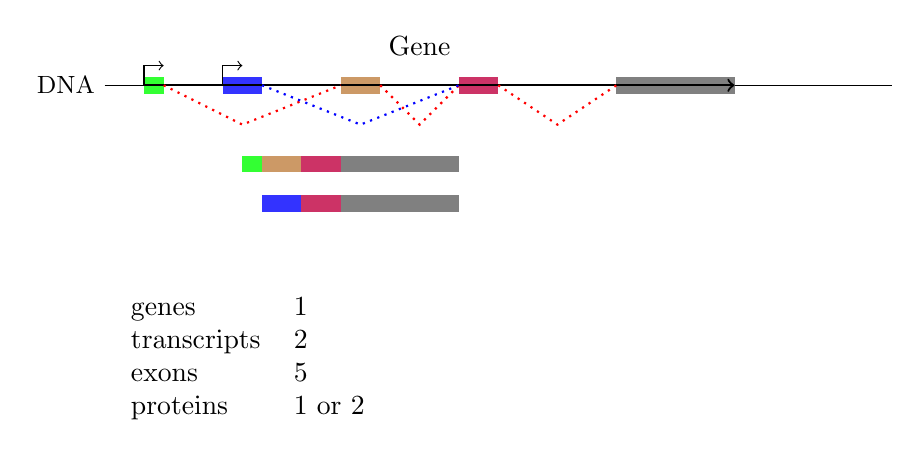
\begin{tikzpicture}[scale=0.5]
%      \draw [help lines] (0,0) grid (20,10);
%      \foreach \x in {1,2,...,20} \node [font=\small] at (\x,0) {\x};
%      \foreach \y in {1,2,...,11} \node [font=\small] at (20,\y) {\y};
      \draw [-, black!100] (0,9) -- (20,9);
      %\visible<1-1>{ }
      \node [left] at (0,9) {\small DNA};
      \visible<2->{
        \draw[green!80, line width=6] (1,9) -- (1.5,9);
        \draw[blue!80, line width=6] (3,9) -- (4,9);
        \draw[brown!80, line width=6] (6,9) -- (7,9);
        \draw[purple!80, line width=6] (9,9) -- (10,9);
        \draw[black!50, line width=6] (13,9) -- (16,9);

        \draw[->] (3,9) -- (3,9.5) -- (3.5,9.5);
        \draw[->] (1,9) -- (1,9.5) -- (1.5,9.5);
        \draw[->, thick] (1,9) -- (16,9);

        \node [above] at (8,9.5) {Gene};
      }

      %splice 1
      \visible<3->{
        \draw[-, red, thick, dotted] (1.5,9) -- ( 3.5,8 ) -- (6,9);
        \draw[-, red, thick, dotted] (7,9) -- (8,8) -- (9,9);
        \draw[-, red, thick, dotted] (10,9) -- (11.5,8) -- (13,9);

        \draw [green!80, line width=6] (3.5,7) -- (4,7);
        \draw [brown!80, line width=6] (4,7) -- (5,7);
        \draw [purple!80, line width=6] (5,7) -- (6,7);
        \draw [black!50, line width=6] (6,7) -- (9,7);
      }
      
      %% splice 2
      \visible<4->{
        \draw [-, blue, thick, dotted] (4,9) -- (6.5,8) -- (9,9);

        \draw [blue!80, line width=6] (4,6) -- (5,6);
        \draw [purple!80, line width=6] (5,6) -- (6,6);
        \draw [black!50, line width=6] (6,6) -- (9,6);
      }

      \visible<5->{
        \node [below right, align=left] at (0,4) {
          \begin{tabular}{ll}
            genes & 1 \\
            transcripts & 2 \\
            exons & 5\\
            proteins & 1 or 2
          \end{tabular}
        };
        }
%          \begin{itemize}
%          \item 1 gene
%          \item 2 transcripts (common exons)
%          \item 5 exons
%          \item 1 or 2 proteins
%          \end{itemize} };
%      }
      
    \end{tikzpicture}
  \end{figure}
\end{frame}

\begin{frame}{Not a tree}
! (gene $\rightarrow$ transcripts $\rightarrow$ exons)

\begin{figure}[ht]
  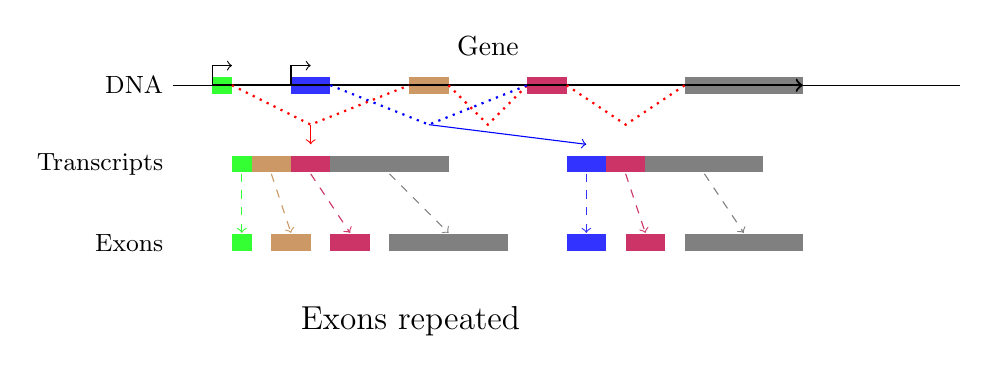
\begin{tikzpicture}[scale=0.5]
%      \draw [help lines, opacity=1] (0,0) grid (22,12);
%      \foreach \x in {1,2,...,20} \node [font=\small] at (\x,0) {\x};
%      \foreach \y in {1,2,...,11} \node [font=\small] at (20,\y) {\y};

      \visible<2->{
      \draw [-, black!100] (0,9) -- (20,9);

      \node [left] at (0,9) {\small DNA};
      \node [left] at (0,7) {\small Transcripts};

      \draw[green!80, line width=6] (1,9) -- (1.5,9);
      \draw[blue!80, line width=6] (3,9) -- (4,9);
      \draw[brown!80, line width=6] (6,9) -- (7,9);
      \draw[purple!80, line width=6] (9,9) -- (10,9);
      \draw[black!50, line width=6] (13,9) -- (16,9);
      
      \draw[->] (3,9) -- (3,9.5) -- (3.5,9.5);
      \draw[->] (1,9) -- (1,9.5) -- (1.5,9.5);
      \draw[->, thick] (1,9) -- (16,9);
      
      \node [above] at (8,9.5) {Gene};

      
      %   splice 1
      \draw[-, red, thick, dotted] (1.5,9) -- ( 3.5,8 ) -- (6,9);
      \draw[-, red, thick, dotted] (7,9) -- (8,8) -- (9,9);
      \draw[-, red, thick, dotted] (10,9) -- (11.5,8) -- (13,9);
      
      \draw [green!80, line width=6] (1.5,7) -- (2,7);
      \draw [brown!80, line width=6] (2,7) -- (3,7);
      \draw [purple!80, line width=6] (3,7) -- (4,7);
      \draw [black!50, line width=6] (4,7) -- (7,7);

      %%   splice 2
      \draw [-, blue, thick, dotted] (4,9) -- (6.5,8) -- (9,9);
      
      \draw [blue!80, line width=6] (10,7) -- (11,7);
      \draw [purple!80, line width=6] (11,7) -- (12,7);
      \draw [black!50, line width=6] (12,7) -- (15,7);

      \draw [->, red] (3.5,8) -- (3.5,7.5);
      \draw [->, blue] (6.5,8) -- (10.5,7.5);
      
      }
      %%  exons 
      \visible<3->{
        \node [left] at (0,5) {\small Exons};
        \draw [green!80, line width=6] (1.5,5) -- (2,5);
        \draw [->, green!80, dashed] (1.75,6.75) -- (1.75,5.25);

        \draw [brown!80, line width=6] (2.5,5) -- (3.5,5);
        \draw [->, brown!80, dashed] (2.5,6.75) -- (3,5.25);

        \draw [purple!80, line width=6] (4,5) -- (5,5);
        \draw [->, purple!80, dashed] (3.5,6.75) -- (4.5,5.25);

        \draw [black!50, line width=6] (5.5,5) -- (8.5,5);
        \draw [->, black!50, dashed] (5.5,6.75) -- (7,5.25);
        
        \draw [blue!80, line width=6] (10,5) -- (11,5);
        \draw [->, blue!80, dashed] (10.5,6.75) -- (10.5,5.25);

        \draw [purple!80, line width=6] (11.5,5) -- (12.5,5);
        \draw [->, purple!80, dashed] (11.5,6.75) -- (12,5.25);

        \draw [black!50, line width=6] (13,5) -- (16,5);
        \draw [->, black!50, dashed] (13.5,6.75) -- (14.5,5.25);
      }
      \visible<4->{
        \node [right] at (3,3) {{\large Exons repeated}};
        }
      
    \end{tikzpicture}
  \end{figure}
\end{frame}

\begin{frame}{core details}
  \begin{figure}[ht]
    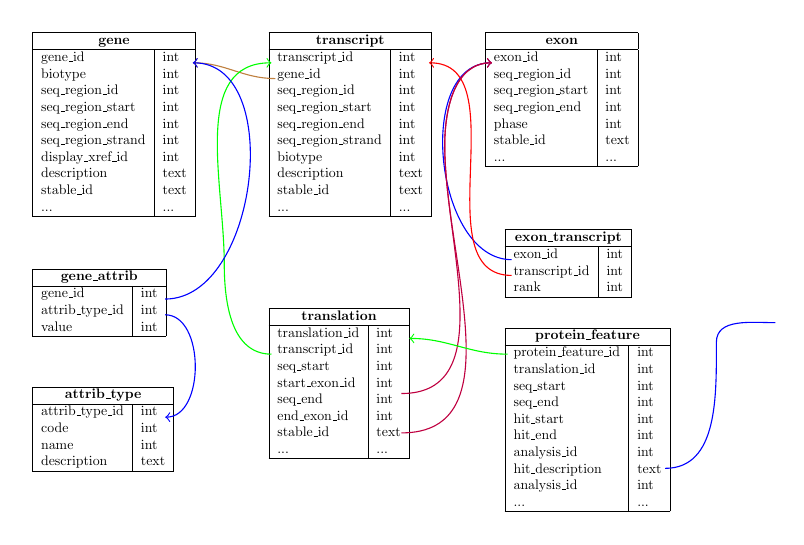
\begin{tikzpicture}[scale=0.5]
%      \draw [help lines, opacity=1] (0,0) grid (22,12);
%      \foreach \x in {1,2,...,20} \node [font=\small] at (\x,0) {\x};
%      \foreach \y in {1,2,...,11} \node [font=\small] at (20,\y) {\y};
      
      \node [below right, align=left, scale=0.5] at (0,12) {
        \begin{tabular}{|l|l|}
          \hline
          \multicolumn{2}{|c|}{\bfseries gene} \\
          \hline
          gene\_id & int \\
          biotype & int \\
          seq\_region\_id & int \\
          seq\_region\_start & int \\
          seq\_region\_end & int \\
          seq\_region\_strand & int \\
          display\_xref\_id & int \\
          description & text \\
          stable\_id & text \\
          ... & ... \\
          \hline
        \end{tabular} };
        
      \node [below right, align=left, scale=0.5] at (6,12) {
        \begin{tabular}{|l|l|}
          \hline
          \multicolumn{2}{|c|}{\bfseries transcript} \\
          \hline
          transcript\_id & int \\
          gene\_id & int \\
          seq\_region\_id & int \\
          seq\_region\_start & int \\
          seq\_region\_end & int \\
          seq\_region\_strand & int \\
          biotype & int \\
          description & text \\
          stable\_id & text \\
          ... & ... \\
          \hline
      \end{tabular} };
      
      \node [below right, align=left, scale=0.5] at (11.5,12) {
        \begin{tabular}{|l|l|}
          \hline
          \multicolumn{2}{|c|}{\bfseries exon} \\
          \hline
          exon\_id & int \\
          seq\_region\_id & int \\
          seq\_region\_start & int \\
          seq\_region\_end & int \\
          phase & int \\
          stable\_id & text \\
          ... & ... \\
          \hline
        \end{tabular} };

      \node [below right, align=left, scale=0.5] at (12,7) {
        \begin{tabular}{|l|l|}
          \hline
          \multicolumn{2}{|c|}{\bfseries exon\_transcript} \\
          \hline
          exon\_id & int \\
          transcript\_id & int \\
          rank & int \\
          \hline
          \end{tabular} };
      \draw [->, blue] (12.3,6.1) to [out=180,in=180] (11.8,11.1);
      \draw [->, red] (12.3,5.7) to [out=180,in=0] (10.2,11.1);
      \draw [->, brown] (6.3,10.7) to [out=180,in=0] (4.2,11.1);
      
      \node [below right, align=left, scale=0.5] at (6,5) {
        \begin{tabular}{|l|l|}
          \hline
          \multicolumn{2}{|c|}{\bfseries translation} \\
          \hline
          translation\_id & int \\
          transcript\_id & int \\
          seq\_start & int \\
          start\_exon\_id & int \\
          seq\_end & int \\
          end\_exon\_id & int \\
          stable\_id & text \\
          ... & ... \\
          \hline
          \end{tabular} };
      
      \draw [->, green] (6.2,3.7) to [out=180,in=270] (5,6) to [out=90,in=180] (6.2,11.1);
      \draw [->, purple] (9.5,2.7) to [out=0,in=270] (10.6,9) to [out=90,in=180] (11.8,11.1);
 
      \draw [->, purple] (9.5,1.7) to [out=0,in=270] (10.6,9) to [out=90,in=180] (11.8,11.1);
            
      
      \node [below right, align=left, scale=0.5] at (12,4.5) {
              \begin{tabular}{|l|l|}
                \hline
          \multicolumn{2}{|c|}{\bfseries protein\_feature} \\
          \hline
          protein\_feature\_id & int \\
          translation\_id & int \\
          seq\_start & int \\
          seq\_end & int \\
          hit\_start & int \\
          hit\_end & int \\
          analysis\_id & int \\
          hit\_description & text \\
          analysis\_id & int \\
          ... & ... \\
          \hline
          \end{tabular} };
      
      \draw [->, green] (12.2,3.7) to [out=180,in=0] (9.7,4.1);
      \draw [-, blue] (16.2,0.8) to [out=0,in=270] (17.5,4) to [out=90,in=180] (19,4.5);
      

      \node [below right, align=left, scale=0.5] at (0,6) {
%        Hello there 

        \begin{tabular}{|l|l|}
          \hline
          \multicolumn{2}{|c|}{\bfseries gene\_attrib} \\
          \hline
          gene\_id & int \\
          attrib\_type\_id & int \\
          value & int \\
          \hline
          \end{tabular} };
      
      \node [below right, align=left, scale=0.5] at (0,3) {
        \begin{tabular}{|l|l|}
          \hline
          \multicolumn{2}{|c|}{\bfseries attrib\_type} \\
          \hline
          attrib\_type\_id & int \\
          code & int \\
          name & int \\
          description & text \\
          \hline
      \end{tabular} };
      
      \draw [->, blue] (3.5,5.1) to [out=0,in=0] (4.2,11.1);
      \draw [->, blue] (3.5,4.7) to [out=0,in=0] (3.5,2.1);

    \end{tikzpicture}
  \end{figure}
\end{frame}

\begin{frame}{full structure}
  
  \tiny \url{http://www.ensembl.org/info/docs/api/core/core_schema.html}
  \begin{figure}[ht]
    \includegraphics[width=\textwidth]{images/ensembl_core_web}
  \end{figure}
\end{frame}

\begin{frame}{how to query}
  Another language to learn:\\
  Structured Query Language \textcolor{blue}{SQL}

  \pause
  Or use a frontend of some sort / web / something else.

  \pause
  My favourite: \texttt{RMySQL} giving direct access to data in R.
\end{frame}

\begin{frame}[fragile]{SQL examples}
  \begin{sqlcode}
SELECT gene_id from gene where stable_id = 'ENSMUSG00002341';

SELECT a.gene_id, b.display_label, a.seq_region_start, 
       a.seq_region_end, a.seq_region_strand
       from gene a
       inner join xref b on a.display_xref_id=b.xref_id;

SELECT c.display_label as symbol, a.stable_id as gene, 
       b.name as chr, d.seq_region_start as start, 
       d.seq_region_end as end, a.seq_region_strand,
       d.transcript_id, d.stable_id as transcript 
       from gene a 
       inner join seq_region b on a.seq_region_id=b.seq_region_id
       inner join xref c on a.display_xref_id=c.xref_id
       inner join transcript d on a.gene_id=d.gene_id
       where c.display_label='nanog';
                   

  \end{sqlcode}
\end{frame}

\begin{frame}[fragile]{table descriptions}
  \begin{sqlcode}
    describe gene;
  \end{sqlcode}

  { \tiny \hspace{-1cm}
\begin{verbatim}
mysql> describe gene;
+-------------------------+----------------------------+------+-----+---------------------+----------------+
| Field                   | Type                       | Null | Key | Default             | Extra          |
+-------------------------+----------------------------+------+-----+---------------------+----------------+
| gene_id                 | int(10) unsigned           | NO   | PRI | NULL                | auto_increment |
| biotype                 | varchar(40)                | NO   |     | NULL                |                |
| analysis_id             | smallint(5) unsigned       | NO   | MUL | NULL                |                |
| seq_region_id           | int(10) unsigned           | NO   | MUL | NULL                |                |
| seq_region_start        | int(10) unsigned           | NO   |     | NULL                |                |
| seq_region_end          | int(10) unsigned           | NO   |     | NULL                |                |
| seq_region_strand       | tinyint(2)                 | NO   |     | NULL                |                |
| display_xref_id         | int(10) unsigned           | YES  | MUL | NULL                |                |
| source                  | varchar(40)                | NO   |     | NULL                |                |
| status                  | enum('KNOWN','NOVEL',...,) | YES  |     | NULL                |                |
| description             | text                       | YES  |     | NULL                |                |
| is_current              | tinyint(1)                 | NO   |     | 1                   |                |
| canonical_transcript_id | int(10) unsigned           | NO   | MUL | NULL                |                |
| stable_id               | varchar(128)               | YES  | MUL | NULL                |                |
| version                 | smallint(5) unsigned       | NO   |     | 1                   |                |
| created_date            | datetime                   | NO   |     | 0000-00-00 00:00:00 |                |
| modified_date           | datetime                   | NO   |     | 0000-00-00 00:00:00 |                |
+-------------------------+----------------------------+------+-----+---------------------+----------------+
17 rows in set (0.00 sec)

\end{verbatim}
}
\end{frame}

\begin{frame}[fragile]{Gene transcripts}
  
  {\tiny
\begin{verbatim}
mysql> select c.display_label as symbol, a.stable_id as gene,
    -> b.name as chr, d.seq_region_start as start, d.seq_region_end as end,
    -> a.seq_region_strand as strand, d.transcript_id, d.stable_id as transcript
    -> from gene a
    -> inner join seq_region b on a.seq_region_id=b.seq_region_id
    -> inner join xref c on a.display_xref_id=c.xref_id
    -> inner join transcript d on a.gene_id=d.gene_id
    -> where c.display_label='cdh5';
+--------+--------------------+-----+----------+----------+--------+---------------+--------------------+
| symbol | gene               | chr | start    | end      | strand | transcript_id | transcript         |
+--------+--------------------+-----+----------+----------+--------+---------------+--------------------+
| cdh1   | ENSDARG00000102750 | 7   | 52827499 | 52847585 |     -1 |         41791 | ENSDART00000167882 |
| cdh1   | ENSDARG00000102750 | 7   | 52788342 | 52847568 |     -1 |         41801 | ENSDART00000168890 |
| cdh1   | ENSDARG00000102750 | 7   | 52826604 | 52847585 |     -1 |         41813 | ENSDART00000172179 |
+--------+--------------------+-----+----------+----------+--------+---------------+--------------------+
3 rows in set (0.00 sec)

\end{verbatim}
}
\end{frame}

\begin{frame}{Too complicated?}
  a little bit complicated, but:
  \begin{itemize}
  \item data can be directly imported into R-sessions, Perl scripts
    and other programs by using packages / libraries / modules.\\
    \textcolor{navy}{\emph{very convenient}}
  \item data can be accessed from disparate locations and users
  \item single location of data
  \item data managed by a system: more difficult to screw things
    up by deleting / moving stuff around
  \item system provides a description of the data structure:\\
    you don't have to keep a note of it on some piece of paper you will lose
  \item complex queries can be stored in scripts / or files. No need
    to redo.
  \item transaction control possible
  \end{itemize}
\end{frame}

\begin{frame}{Mutability?}
  We can also divide databases by their usage:
  \begin{itemize}
  \item Read only, or primarily read only databases. These
    are filled with data on creation and the data is used, but
    only rarely modified. A typical example are the genome databases
    like Ensembl.
  \item Incremental databases are still primarily read only, but
    users are able to add data to the system through standardised
    interfaces but data should never be modified (eg. genbank).
  \item Transaction databases. These are used for things like recording
    reservations and are in constant flux and must be built with adequate
    transaction controls in place (e.g. make sure two people don't book
    the same seat, one person gets two salaries...). A laboratory data
    management system would also be an example of such (reagents running out,
    being purchased, etc...).
  \end{itemize}
  
  \blfootnote{There is an argument that databases should never modify data,
    but modify meaning by adding records, but lets not get into details.}
\end{frame}

\begin{frame}{but, I'm too lazy for all this}
  Not always necessary to build database systems for what you are doing, but:

  Do think about formalising the relationships between your data points (both
  input and output). This helps to understand the nature of what you are doing.

  if nothing else: may lead you to a rational way of labelling your tubes.
\end{frame}

\end{document}
